% Options for packages loaded elsewhere
\PassOptionsToPackage{unicode}{hyperref}
\PassOptionsToPackage{hyphens}{url}
\documentclass[
]{article}
\usepackage{xcolor}
\usepackage{amsmath,amssymb}
\setcounter{secnumdepth}{-\maxdimen} % remove section numbering
\usepackage{iftex}
\ifPDFTeX
  \usepackage[T1]{fontenc}
  \usepackage[utf8]{inputenc}
  \usepackage{textcomp} % provide euro and other symbols
\else % if luatex or xetex
  \usepackage{unicode-math} % this also loads fontspec
  \defaultfontfeatures{Scale=MatchLowercase}
  \defaultfontfeatures[\rmfamily]{Ligatures=TeX,Scale=1}
\fi
\usepackage{lmodern}
\ifPDFTeX\else
  % xetex/luatex font selection
\fi
% Use upquote if available, for straight quotes in verbatim environments
\IfFileExists{upquote.sty}{\usepackage{upquote}}{}
\IfFileExists{microtype.sty}{% use microtype if available
  \usepackage[]{microtype}
  \UseMicrotypeSet[protrusion]{basicmath} % disable protrusion for tt fonts
}{}
\makeatletter
\@ifundefined{KOMAClassName}{% if non-KOMA class
  \IfFileExists{parskip.sty}{%
    \usepackage{parskip}
  }{% else
    \setlength{\parindent}{0pt}
    \setlength{\parskip}{6pt plus 2pt minus 1pt}}
}{% if KOMA class
  \KOMAoptions{parskip=half}}
\makeatother
\usepackage{graphicx}
\makeatletter
\newsavebox\pandoc@box
\newcommand*\pandocbounded[1]{% scales image to fit in text height/width
  \sbox\pandoc@box{#1}%
  \Gscale@div\@tempa{\textheight}{\dimexpr\ht\pandoc@box+\dp\pandoc@box\relax}%
  \Gscale@div\@tempb{\linewidth}{\wd\pandoc@box}%
  \ifdim\@tempb\p@<\@tempa\p@\let\@tempa\@tempb\fi% select the smaller of both
  \ifdim\@tempa\p@<\p@\scalebox{\@tempa}{\usebox\pandoc@box}%
  \else\usebox{\pandoc@box}%
  \fi%
}
% Set default figure placement to htbp
\def\fps@figure{htbp}
\makeatother
\setlength{\emergencystretch}{3em} % prevent overfull lines
\providecommand{\tightlist}{%
  \setlength{\itemsep}{0pt}\setlength{\parskip}{0pt}}
\usepackage{bookmark}
\IfFileExists{xurl.sty}{\usepackage{xurl}}{} % add URL line breaks if available
\urlstyle{same}
\hypersetup{
  pdftitle={Reference-relative believability in photoreal human avatars: synthetic identity as a systems constraint},
  pdfauthor={D. B. Havery},
  hidelinks,
  pdfcreator={LaTeX via pandoc}}

\title{Reference-relative believability in photoreal human avatars:
synthetic identity as a systems constraint}
\author{D. B. Havery}
\date{}

\begin{document}
\maketitle

\emph{D. B. Havery. Manuscript draft, v0.3 (2026-07-02).} \emph{Intended
classification: Human-computer interaction; computer graphics; computer
vision; applied AI systems. Keywords: photoreal avatars, synthetic human
identity, full-body generation, conversational agents, talking-head
synthesis, uncanny valley, familiar face perception, identity, system
design.}

\subsection{Abstract}\label{abstract}

Photoreal avatars are usually treated as renderer problems: make the
generated human sharp enough, stable enough, and temporally coherent
enough to pass as video. That account is incomplete. Avatar quality is
judged relative to the reference implied by the product. For a known
real person, the reference is the viewer\textquotesingle s stored model
of that person\textquotesingle s appearance and motion. For a persistent
synthetic character, the reference is the system\textquotesingle s
canonical identity state: face, body, voice, styling range, provenance,
and continuity contract. For a one-off synthetic stranger, the reference
is the broader human category. I define this dependency as
reference-relative believability and use ground-truth drift for
deviation from the applicable reference. The distinction yields testable
predictions: familiarity-dependent rejection for known real people,
continuity-dependent rejection for persistent synthetic identities,
full-body exposure effects, and latency-fidelity tradeoffs between live
interaction and close inspection. It also changes system design. The
split is not known person versus invented person. It is high-fidelity
identity path versus live interaction path. A prototype Avatar Engine
implements this boundary with character registries, renderer routing, a
local real-time talking-head loop, and separate high-fidelity
identity-planning work for synthetic human rosters. The implementation
is not perceptual validation, but it shows that the boundary is concrete
enough to build.

\subsection{1. Introduction}\label{1-introduction}

Photoreal avatar systems now combine several capabilities that are often
discussed separately: image generation, full-body rendering,
talking-head animation, speech recognition, language models, speech
synthesis, memory, and browser or device transport. The product promise
is larger than a face that talks. A mature avatar engine should support
assistants, support agents, virtual friends, presenters, content
creation, and persistent virtual talent for modeling or campaign work.

That product promise exposes a constraint that renderer-centric accounts
miss. Most valuable avatars are not intended to copy one real person.
They are authored synthetic identities. The target is still strict: a
made-up character should be indistinguishable from a real human when
that is the product claim, and it should remain the same character
across sessions, poses, outfits, lighting, camera positions, and future
model upgrades. The absence of a real-person original does not remove
the reference problem. It moves the reference into the system.

The build history that motivated this manuscript began with a reusable
Avatar Engine: character + voice + model + persona as a live interface.
Early iterations treated known-person likenesses, support agents,
assistants, presenters, and full-body synthetic characters as variants
of the same rendering problem. That abstraction failed. Digital-double
reconstruction, blendshape bridges, procedural idle motion, single-image
reenactment, and mouth-only lip-sync failed in different ways. Later
full-body experiments widened the failure surface: skin texture, eye
highlights, hands, hair, face pixel size, body proportions, garment
interaction, pose, and lighting became as important as lips or teeth.

I use reference-relative believability for the resulting principle.
Avatar outputs are judged against the reference implied by the task. A
known real person is judged against the viewer\textquotesingle s stored
model. A persistent synthetic character is judged against its canonical
identity state. A one-off synthetic stranger is judged against the
real-human category. Ground-truth drift is deviation from whichever
reference applies.

This distinction changes the architecture. The practical split is not
real person versus invented person. It is high-fidelity identity path
versus live interaction path. The former is for artifacts expected to
survive high-definition, close human inspection. The latter is for
conversational presence, where latency and turn-taking are part of
quality. Known-person likeness is one strict case inside the
high-fidelity path, not the whole problem.

The claims are limited and testable:

\begin{enumerate}
\def\labelenumi{\arabic{enumi}.}
\tightlist
\item
  It defines reference-relative believability and ground-truth drift for
  photoreal human avatars, including persistent synthetic identities.
\item
  It predicts familiarity, continuity, and full-body exposure effects
  that a renderer-only account does not predict.
\item
  It derives an identity-contract architecture that separates
  high-fidelity identity rendering from live interaction while
  preserving a shared conversational stack.
\end{enumerate}

\subsection{2. Background and related
work}\label{2-background-and-related-work}

\subsubsection{2.1 Uncanny valley and cue
inconsistency}\label{21-uncanny-valley-and-cue-inconsistency}

Mori\textquotesingle s uncanny valley gives the familiar shape of the
problem: affinity drops when an entity becomes nearly, but not fully,
human {[}1{]}. Later accounts sharpen the mechanism by emphasizing
motion, category conflict, and prediction error {[}2, 3{]}. Those
accounts explain why a stimulus can feel wrong. They do not, by
themselves, explain why the same renderer can be tolerable in one
product context and intolerable in another. The missing variable is not
only in the pixels. It is the reference the output is expected to
satisfy. Recent avatar studies are consistent with this: controlled
experiments show that perceived naturalness and eeriness depend on the
consistency of realism cues and on the interaction context rather than
on raw fidelity alone {[}14{]}, and a network meta-analysis of
avatar-realism studies finds that the effect of appearance realism on
perceptual experience is moderated by task and setting {[}15{]}.

\subsubsection{2.2 Familiar and self-face
perception}\label{22-familiar-and-self-face-perception}

Familiar-face research supplies the known-person asymmetry. Familiar
faces are processed differently from unfamiliar faces {[}4, 5{]}, and
people recognize them under degraded conditions that defeat
unfamiliar-face recognition {[}6, 7{]}. Self-face processing is also
special {[}8{]}. In recognition tasks, this robustness is an advantage.
In synthesis, it can become a liability. The same stored model that lets
a viewer recognize a poor recording of a familiar person also gives them
a sharper target for rejecting an almost-correct reconstruction. Recent
synthetic-media work supplies converging evidence: a systematic review
of human deepfake detection finds that familiarity with the depicted
person improves detection of manipulated faces, moderated by generation
quality and by whether the depicted behavior is plausible for that
person {[}16{]}. The known-person asymmetry this manuscript predicts is
therefore not hypothetical; it already appears in detection studies as a
familiarity advantage that a synthesis system must overcome.

\subsubsection{2.3 Talking-head and portrait animation
systems}\label{23-talking-head-and-portrait-animation-systems}

Talking-head systems generate or retarget facial motion from speech,
images, video, or learned motion spaces {[}9-12{]}. Newer unified
audio-to-video systems suggest that live avatar quality will keep
improving {[}13{]}. The point here is not that these systems are weak.
The point is that many systems optimize a narrow face crop or a short
video window, while product-grade avatars may require full-body
identity, garment realism, continuity across shoots, and close
inspection. Small losses in skin texture, mouth detail, hand anatomy,
head motion, gaze, or temporal consistency have different costs
depending on the reference contract.

\subsubsection{2.4 Synthetic identity, provenance, and
presence}\label{24-synthetic-identity-provenance-and-presence}

Three further literatures bear on the reference argument. First, the
deepfake and face-swap literature is, in effect, the study of identity
judged against an external reference; its central finding â€'' that
viewers detect manipulation better when the identity is familiar
{[}16{]} â€'' is the known-person case of reference-relative
believability stated in detection terms. Second, content-provenance
efforts such as the C2PA Content Credentials specification attach
cryptographically signed origin and edit history to media {[}17{]}.
Provenance is orthogonal to perceptual realism, but it is the mechanism
by which a system can bind an output to a declared reference and
continuity contract, which is exactly what the architecture in Section 6
enforces at the renderer boundary. Third, work on avatar realism and
social presence shows that acceptance depends on immersion, task, and
interaction context, not fidelity in isolation {[}14, 15{]}, which is
why this manuscript separates a close-inspection realism bar from a
live-presence bar rather than collapsing both into one "photoreal"
score.

\subsection{3. Definitions}\label{3-definitions}

Five terms carry the argument.

\textbf{Reference.} A reference is the target against which the avatar
is judged. It may be external viewer memory of a real person, an
internal canonical identity state for a synthetic character, or the
broader category of real human appearance and motion.

\textbf{Known-person reference.} A known-person reference exists when
the product claim requires acceptance as a known real human. Examples
include a user\textquotesingle s own likeness, a
company\textquotesingle s real spokesperson, or a public figure.
Deviations from the stored reference are identity errors, not merely
artifacts.

\textbf{Canonical synthetic identity.} A canonical synthetic identity is
an authored character with durable system state: face, body, voice,
styling range, identity references, provenance, policy, and continuity
thresholds. It is not copied from one real person, but it still has a
reference once saved and reused.

\textbf{One-off synthetic stranger.} A one-off synthetic stranger is an
invented human image or clip with no durable identity contract. It must
still satisfy the real-human category bar, but it is not yet responsible
for continuity across future uses.

\textbf{Ground-truth drift.} Ground-truth drift is deviation from the
applicable reference. For a known person, drift is mismatch with viewer
memory. For a canonical synthetic identity, drift is mismatch with the
stored identity contract. For a one-off stranger, drift is failure to
belong convincingly to the real-human category.

\textbf{Reference-relative believability.} Reference-relative
believability is the claim that perceived avatar quality is a function
of generated output quality, reference strength, task context, and
inspection level. In simplified form:

\begin{quote}
perceived believability = f(render quality, reference strength, task
context, inspection level)
\end{quote}

This expression is schematic, not a fitted model. It names the factors
the account holds responsible; their operational measures and the
statistical model that relates them are given in Section 5.2 and 5.3.
The contribution is the set of factors and their predicted interactions,
not a specific functional form.

The claim does not imply that synthetic identities are automatically
believable. They can fail through ordinary artifacts: unstable geometry,
dead eyes, poor lip sync, incoherent lighting, waxy skin, broken hands,
body inconsistency, or temporal jitter. The claim is narrower: different
references create different error budgets.

\subsection{4. Hypotheses}\label{4-hypotheses}

If the account is right, user ratings move in specific ways.

\textbf{H1: familiarity gradient.} For the same synthesis pipeline and
artifact level, naturalness ratings will decrease as viewer familiarity
with a depicted real person increases.

\textbf{H2: self-recognition ceiling.} Self-avatar clips will be
rejected at fidelity levels that the same viewers accept for unfamiliar
humans or newly authored synthetic identities.

\textbf{H3: synthetic rescue with decay.} A synthesis pipeline judged
unacceptable for a known person\textquotesingle s likeness will receive
higher naturalness and acceptance ratings when the identity is replaced
with a newly authored synthetic identity, holding rendering method,
framing, prompt content, and voice quality as constant as possible. The
advantage should shrink after the synthetic identity is made persistent
and repeatedly shown to raters.

\textbf{H4: continuity-contract penalty.} Persistent synthetic
identities will be rejected more often than one-off synthetic strangers
when outputs drift from a canonical reference set, even if independent
raters score the visible artifacts similarly.

\textbf{H5: full-body exposure effect, with a reference interaction.}
Moving from headshot or bust framing to full-body framing will increase
rejection because it exposes hands, hair, body proportions, garment
interaction, face-pixel limits, pose, and lighting coherence. The
non-obvious prediction is the interaction: the full-body penalty will be
larger for persistent synthetic identities and known people than for
one-off strangers, because the added surface must match a stored
reference (a saved body state or viewer memory), not merely belong to
the human category. A one-off stranger only has to look plausibly human
at full body; a persistent identity has to look like the same body it
established earlier.

\textbf{H6: latency-fidelity trade.} Live interaction paths will score
better on perceived responsiveness and presence, while gated
high-fidelity paths will score better on close-inspection realism and
identity continuity.

These hypotheses can fail. If viewer familiarity does not affect
naturalness or "not them" judgments after controlling for visible
artifact severity, the known-person mechanism is wrong or incomplete. If
persistent synthetic identities are not penalized for continuity drift,
the canonical-reference mechanism is wrong or incomplete.

\subsection{5. Evaluation protocol}\label{5-evaluation-protocol}

A minimal study can use existing synthesis pipelines. The important move
is to hold the renderer fixed and vary the identity relation between
clip and rater.

\subsubsection{5.1 Stimuli}\label{51-stimuli}

The stimulus set needs four classes:

\begin{enumerate}
\def\labelenumi{\arabic{enumi}.}
\tightlist
\item
  \textbf{Known-person clips.} Synthesized clips of subjects for whom a
  subset of raters has direct familiarity.
\item
  \textbf{Unfamiliar real-person clips.} Synthesized clips of real
  people unknown to the raters.
\item
  \textbf{New synthetic-identity clips.} Synthesized clips of authored
  identities with no prior exposure to raters.
\item
  \textbf{Persistent synthetic-identity clips.} Synthesized clips or
  images of authored identities after raters have been shown a canonical
  reference set.
\end{enumerate}

Duration, framing, lighting, prompt content, voice quality, and output
resolution are held constant where possible. The study should include
both headshot and full-body conditions. If known-person voice cloning is
used, voice familiarity must be modeled separately because voice carries
its own reference.

\subsubsection{5.2 Measures}\label{52-measures}

Each rater supplies:

\begin{enumerate}
\def\labelenumi{\arabic{enumi}.}
\tightlist
\item
  Naturalness rating.
\item
  Identity acceptance rating for known-person and persistent synthetic
  clips.
\item
  "Not quite them" judgment for known-person clips and "not the same
  character" judgment for persistent synthetic clips.
\item
  Comfort or uncanny-valley rating.
\item
  Free-text artifact description.
\item
  Familiarity rating for the depicted identity or exposure count for
  synthetic identities.
\item
  Confidence in judgment.
\end{enumerate}

Artifact severity is rated by a separate group that does not know the
depicted identities. That separates visible defects from
familiarity-driven rejection.

\subsubsection{5.3 Analysis}\label{53-analysis}

The primary model treats acceptance as a function of identity condition,
viewer familiarity or exposure, artifact severity, framing, inspection
level, and their interactions. A mixed-effects model is the natural fit
because both clips and raters repeat. The key tests are whether
familiarity predicts lower acceptance for known-person clips after
artifact severity is included, and whether canonical exposure predicts
lower tolerance for continuity drift in persistent synthetic identities.

\subsubsection{5.4 Expected result
pattern}\label{54-expected-result-pattern}

The reference-relative account predicts the following ordering, from
easiest to hardest, assuming comparable artifact severity:

\begin{enumerate}
\def\labelenumi{\arabic{enumi}.}
\tightlist
\item
  One-off synthetic stranger.
\item
  Unfamiliar real person.
\item
  Newly authored synthetic identity.
\item
  Persistent synthetic identity with a canonical reference set.
\item
  Weakly familiar public figure.
\item
  Personally familiar person.
\item
  Self-avatar.
\end{enumerate}

This ordering is not a moral or legal ranking. It is a perceptual
error-budget ranking. Safety, consent, provenance, and labeling
requirements may be strict in every tier.

\subsection{6. System architecture}\label{6-system-architecture}

In an implementation, the claim becomes a router. The conversational
stack can be shared, but the render path is selected by identity
contract, inspection bar, latency target, and provenance requirement.

\pandocbounded{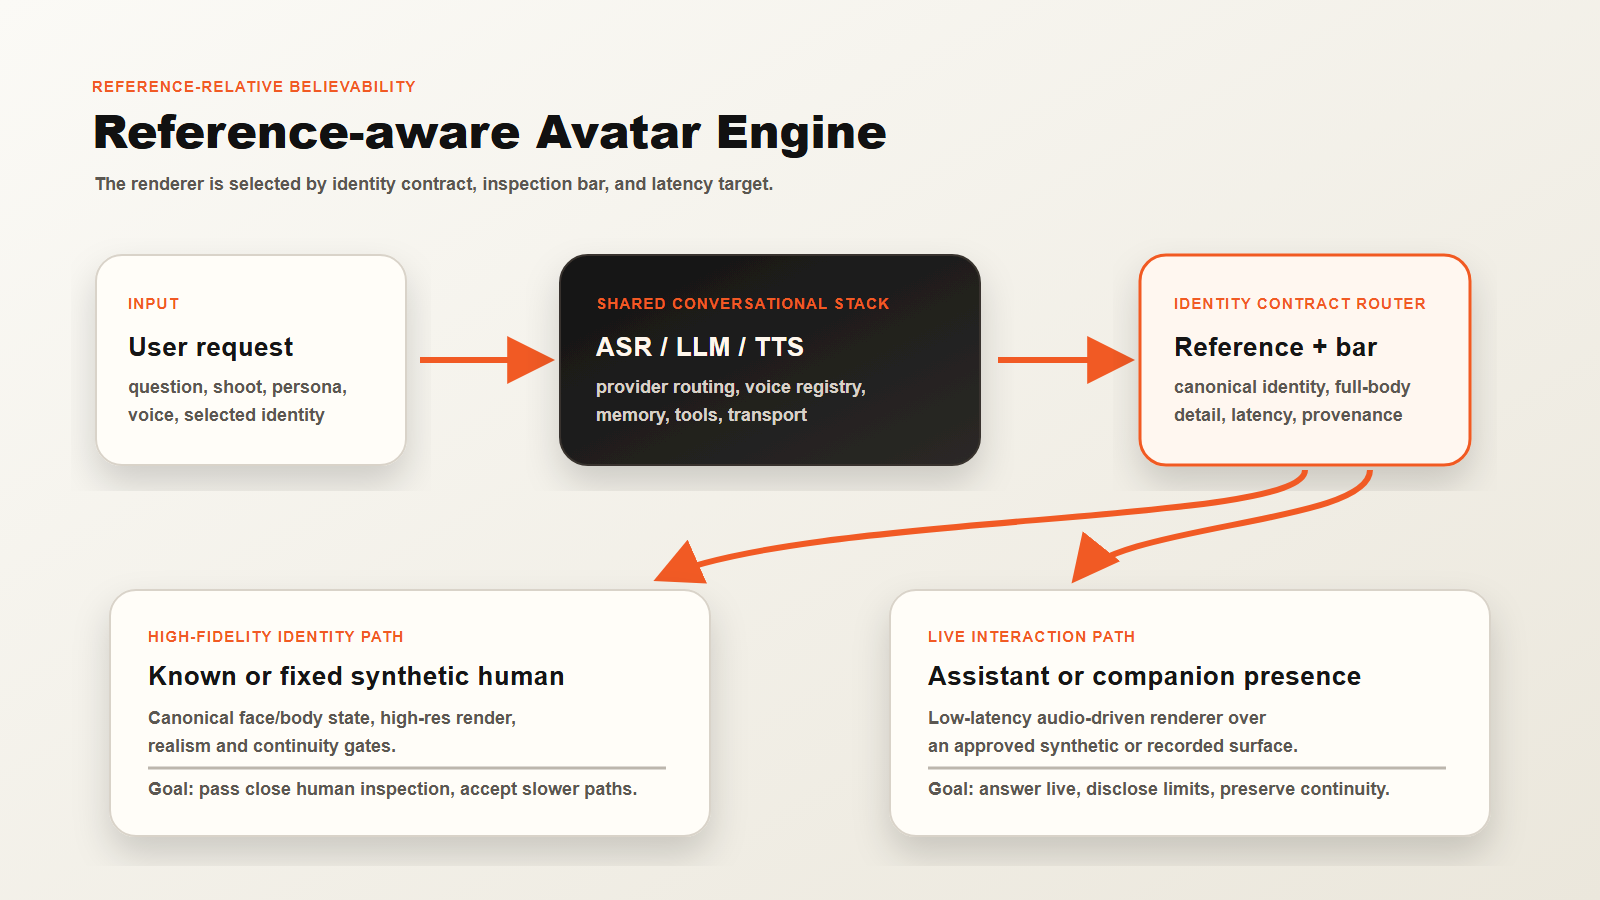
\includegraphics[keepaspectratio,alt={Reference-aware Avatar Engine architecture. Shared conversational systems feed an identity contract router; high-fidelity identities use gated render paths, while live interaction surfaces use low-latency render paths.}]{assets/two-tier-avatar-engine.png}}

\emph{Figure 1. Reference-aware Avatar Engine architecture. The
conversational stack is shared, but the renderer is selected by identity
contract, inspection bar, latency target, and provenance requirement.}

The shared stack includes speech recognition, language model, tools,
memory, voice selection, transport, and policy controls. None of these
components necessarily changes the identity surface. The identity
contract router is the boundary where visual identity becomes a systems
constraint.

High-fidelity identity requests route to a gated render path. For known
people, that may mean recorded footage, constrained playback, or narrow
edits that preserve the recorded identity surface. For canonical
synthetic identities, it means high-resolution generation, full-body
realism gates, continuity checks, provenance, and human review for
uncertain cases. This path may sacrifice latency to protect identity and
close-inspection realism.

Live interaction requests route to a low-latency path: talking-head
renderers, audio-driven animation, pre-rendered idle clips, or streaming
video chunks. This path optimizes responsiveness and presence while
preserving the character registry and policy contract. It should not be
represented as proof of full-body indistinguishability unless it clears
that separate gate.

Registry design changes too: a character carries identity provenance,
canonical state, allowed renderers, voice policy, continuity thresholds,
disclosure rules, and safety constraints. This prevents a high-fidelity
identity from entering an inappropriate renderer and prevents a
low-latency surface from making claims it cannot satisfy.

Figure 1 draws the shared stack as a cascade of speech recognition,
language model, and speech synthesis, but the argument does not depend
on that decomposition. Emerging end-to-end systems collapse the cascade
into a single model that jointly perceives and generates synchronized
audio and video at sub-second latency {[}13{]}. Such a system replaces
the low-latency render path, not the identity contract.
Reference-relative believability is a claim about the relation between
an output and the reference a viewer or system holds; it is indifferent
to whether that output is produced by a cascade or by one unified model.
A unified model still needs to be told which identity it may present,
whether the result must clear a full-body close-inspection gate, and
which provenance and continuity rules apply. The router therefore sits
above the renderer regardless of the renderer\textquotesingle s internal
architecture, and a more capable live renderer raises the live-presence
score without, by itself, discharging the separate high-fidelity
identity bar.

\subsection{7. Implementation
feasibility}\label{7-implementation-feasibility}

A private Avatar Engine prototype implements the split. This section is
a feasibility argument, not perceptual validation and not an
independently verifiable benchmark: it shows that the identity boundary
can be expressed as concrete data contracts and enforced in code, which
is what distinguishes an architectural claim from a slide label. Because
the prototype is not yet public, the details below should be read as an
existence argument that the boundary is buildable, not as a measured
result. The relevant details are concrete:

\begin{enumerate}
\def\labelenumi{\arabic{enumi}.}
\tightlist
\item
  The Python package defines character, voice, language-model, and
  renderer registries.
\item
  Character records carry tier and visibility constraints.
\item
  Renderers sit behind a fixed \texttt{RenderEngine} provider protocol.
\item
  A Ditto-backed provider drives the low-latency talking-head path.
\item
  A local conversational loop connects speech recognition, an Ollama
  language model, Piper voice synthesis, and the renderer.
\item
  TensorRT acceleration on the Ditto path reaches the real-time
  interaction tier on local GPU hardware.
\item
  A resident worker keeps the renderer warm, and a streaming path
  renders answer chunks as they complete.
\item
  Separate high-fidelity planning work defines synthetic identity
  creation, roster state, full-body variation grids, realism gates,
  continuity services, provenance records, and human review.
\end{enumerate}

The prototype does not close the product. Full-duplex barge-in, idle
motion, latency tuning, full-body video, garment transfer, and
large-scale perceptual validation remain open engineering work. The
important point is narrower: the identity split is not a slide label. It
is represented in data contracts and enforced at the registry and
renderer boundary.

\subsection{8. Design implications}\label{8-design-implications}

The identity-contract split changes the product specification.
"Photoreal" is not enough. A requirement has to state which reference
the avatar must satisfy: known-person memory, canonical synthetic
identity, or one-off human realism.

It also changes benchmarks. Category-level realism, canonical identity
continuity, known-person likeness, full-body close-inspection realism,
and conversational presence belong in separate scores. A renderer can be
good enough for a live assistant and still unacceptable for a full-body
virtual model. Conversely, a slower gated render path can be correct for
high-fidelity identity work even if it gives up real-time interaction.

Identity provenance belongs in the render contract. The renderer needs
to know whether it is allowed to synthesize the identity surface,
whether the output must pass full-body gates, whether the character is
persistent, and which disclosure requirements apply. This is not a
user-interface detail; it is part of the safety boundary.

\subsection{9. Safety and ethics}\label{9-safety-and-ethics}

Reference-relative believability is not an argument for easier
deployment of synthetic people. Synthetic humans can manipulate,
mislead, create false impressions of agency, or be misused even when
they do not copy one real person. Known-person likeness raises
additional consent and impersonation concerns because it invokes an
external real identity.

The identity distinction belongs in the system, not in copy or policy
language alone. Known-person identities require provenance, consent,
disclosure, and renderer constraints. Signed content-provenance
standards such as C2PA Content Credentials {[}17{]} give a concrete
transport for the provenance and disclosure fields the identity contract
carries, though they do not by themselves prevent misuse and can be
stripped in re-encoding. Persistent synthetic identities still need
labeling, source-safety rules, similarity checks, age safeguards,
continuity records, and audit logs, especially in support, sales,
education, medical, modeling, or companion contexts.

The architecture also reduces accidental misuse. If identity contracts
constrain renderer access, a product is less likely to convert a real
person\textquotesingle s likeness into an unconstrained speaking agent
or let a persistent synthetic identity drift through configuration
changes.

\subsection{10. Limitations}\label{10-limitations}

This manuscript does not report a completed human-subjects study. Its
contribution is a framework, a set of falsifiable predictions, and a
pre-registration-ready evaluation protocol (Section 5), not an empirical
result; it should be read and judged as such. The hypotheses are
testable, but the empirical curve remains open. The proposed gradients
may vary by culture, task, screen size, exposure duration, artifact
type, and inspection condition.

The distinction between one-off and persistent synthetic identities can
also blur. A synthetic character used for a long time may become
familiar to users, creating a new viewer-side reference. A public
synthetic character may acquire a stable identity that future renderers
must preserve. The tier model should therefore be treated as a starting
condition and governance rule, not a permanent guarantee.

Future renderers may reduce visible drift enough that the thresholds
move. The claim does not depend on today\textquotesingle s artifacts
being permanent. It depends on the comparison relation between output
and viewer. If that relation stops predicting acceptance, the theory has
to change.

\subsection{11. Conclusion}\label{11-conclusion}

Photoreal avatars are not one fidelity problem. A one-off synthetic
stranger must look like a real human. A persistent synthetic identity
must also remain the same character across contexts. A known-person
likeness must remain correct relative to viewer memory. A live assistant
must answer quickly enough to feel present. These requirements impose
different error budgets and should not be routed through one
undifferentiated renderer. Reference-relative believability explains why
the practical architecture should split high-fidelity identity work from
live interaction. That design does not solve every avatar problem, but
it avoids forcing one system to satisfy incompatible perceptual
contracts.

\subsection{References}\label{references}

{[}1{]} M. Mori, "The uncanny valley," \emph{Energy}, vol. 7, no. 4, pp.
33-35, 1970. Trans. K. F. MacDorman and N. Kageki, \emph{IEEE Robotics
\& Automation Magazine}, vol. 19, no. 2, pp. 98-100, 2012.

{[}2{]} A. P. Saygin, T. Chaminade, H. Ishiguro, J. Driver, and C.
Frith, "The thing that should not be: predictive coding and the uncanny
valley in perceiving human and humanoid robot actions," \emph{Social
Cognitive and Affective Neuroscience}, vol. 7, no. 4, pp. 413-422, 2012.

{[}3{]} R. K. Moore, "A Bayesian explanation of the
\textquotesingle uncanny valley\textquotesingle{} effect and related
psychological phenomena," \emph{Scientific Reports}, vol. 2, art. 864,
2012.

{[}4{]} V. Bruce and A. Young, "Understanding face recognition,"
\emph{British Journal of Psychology}, vol. 77, no. 3, pp. 305-327, 1986.

{[}5{]} R. A. Johnston and A. J. Edmonds, "Familiar and unfamiliar face
recognition: a review," \emph{Memory}, vol. 17, no. 5, pp. 577-596,
2009.

{[}6{]} A. M. Burton, S. Wilson, M. Cowan, and V. Bruce, "Face
recognition in poor-quality video: evidence from security surveillance,"
\emph{Psychological Science}, vol. 10, no. 3, pp. 243-248, 1999.

{[}7{]} P. J. B. Hancock, V. Bruce, and A. M. Burton, "Recognition of
unfamiliar faces," \emph{Trends in Cognitive Sciences}, vol. 4, no. 9,
pp. 330-337, 2000.

{[}8{]} F. Tong and K. Nakayama, "Robust representations for faces:
evidence from visual search," \emph{Journal of Experimental Psychology:
Human Perception and Performance}, vol. 25, no. 4, pp. 1016-1035, 1999.

{[}9{]} K. R. Prajwal, R. Mukhopadhyay, V. P. Namboodiri, and C. V.
Jawahar, "A lip sync expert is all you need for speech to lip generation
in the wild" (Wav2Lip), in \emph{Proc. ACM Int. Conf. Multimedia (MM)},
2020, pp. 484-492.

{[}10{]} J. Guo et al., "LivePortrait: efficient portrait animation with
stitching and retargeting control," arXiv:2407.03168, 2024.

{[}11{]} T. Li, R. Zheng, M. Yang, J. Chen, and M. Yang, "Ditto:
motion-space diffusion for controllable realtime talking head
synthesis," arXiv:2411.19509, 2024 (ACM MM 2025).

{[}12{]} S. Xu et al., "VASA-1: lifelike audio-driven talking faces
generated in real time," in \emph{Advances in Neural Information
Processing Systems (NeurIPS)}, 2024. arXiv:2404.10667.

{[}13{]} Wan Team, Alibaba Group, "Wan-Streamer v0.1: end-to-end
real-time interactive foundation models," arXiv:2606.25041, 2026.

{[}14{]} T. D. Do, R. P. McMahan, and P. J. Wisniewski, "A new uncanny
valley? The effects of speech fidelity and human listener gender on
social perceptions of a virtual-human speaker," in \emph{Proc. CHI Conf.
Human Factors in Computing Systems (CHI \textquotesingle22)}, 2022.

{[}15{]} Z. Tao, Y. Liu, J. Qiu, and S. Li, "Impact of virtual avatar
appearance realism on perceptual interaction experience: a network
meta-analysis," \emph{Frontiers in Psychology}, vol. 16, art. 1624975,
2025.

{[}16{]} K. Somoray, D. Miller, and M. Holmes, "Human performance in
deepfake detection: a systematic review," \emph{Human Behavior and
Emerging Technologies}, 2025, doi:10.1155/hbe2/1833228.

{[}17{]} Coalition for Content Provenance and Authenticity, "C2PA
technical specification (Content Credentials)," version 2.2, 2025.
{[}Online{]}. Available: \url{https://c2pa.org/specifications/}

\end{document}
